66. На координатной плоскости изображены графики функций $y=(x^2-9)(x^2-4)(x-1)(x-2)+7x-12x^2$ и $y=-50(|1-|2|x|-4||-1)+7x-12x^2$ при
$x\in[-2,5;3,1].$\\
a. Установите, график какой из функций синий, а какой --- красный. Ответ обоснуйте.\\
b. Решите неравенство  $-50(|1-|2|x|-4||-1)+7x-12x^2 >(x^2-9)(x^2-4)(x-1)(x-2)+7x-12x^2$ при
$x\in[-2,5;3]$ и запишите ответ (обоснование не требуется).
\begin{center}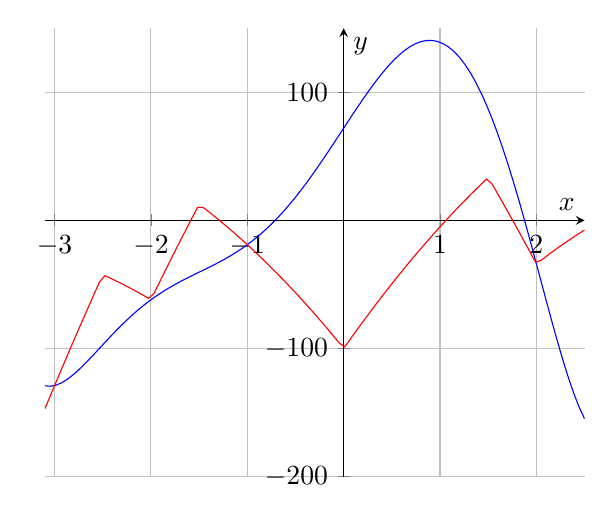
\begin{tikzpicture}[scale=1]
\begin{axis}[
    axis lines = middle,
    grid=both,
    legend pos={south west},
    xlabel = {$x$},
    %xlabel style={below right},
    ylabel = {$y$},
    ymin=-200,
    ymax=150
               ]
	\addplot[domain=-3.1:2.5, samples=100, color=blue] {(x^2-9)*(x^2-4)*(x+1)*(x+2)+7*x-12*x^2};
\addplot[domain=-3.1:2.5, samples=100, color=red] {-50*(abs(1-abs(2*abs(x)-4))-1)+7*x-12*x^2};
	
\end{axis}
\end{tikzpicture}\end{center}
